% Exam Template for UMTYMP and Math Department courses
%
% Using Philip Hirschhorn's exam.cls: http://www-math.mit.edu/~psh/#ExamCls
%
% run pdflatex on a finished exam at least three times to do the grading table on front page.
%
%%%%%%%%%%%%%%%%%%%%%%%%%%%%%%%%%%%%%%%%%%%%%%%%%%%%%%%%%%%%%%%%%%%%%%%%%%%%%%%%%%%%%%%%%%%%%%

% These lines can probably stay unchanged, although you can remove the last
% two packages if you're not making pictures with tikz.
\documentclass[11pt]{exam}
\RequirePackage{amssymb, amsfonts, amsmath, latexsym, verbatim, xspace, setspace}
\RequirePackage{tikz, pgflibraryplotmarks}

% By default LaTeX uses large margins.  This doesn't work well on exams; problems
% end up in the "middle" of the page, reducing the amount of space for students
% to work on them.
\usepackage[margin=1in]{geometry}
\usepackage{etoolbox}

\newtoggle{hideans}
\toggletrue{hideans}


% Here's where you edit the Class, Exam, Date, etc.
\newcommand{\class}{Physics 121}
\newcommand{\term}{Fall 2017}
\newcommand{\examnum}{Exam 1}
\newcommand{\examdate}{19 Sep 2017}
\newcommand{\timelimit}{60 Minutes}

% For an exam, single spacing is most appropriate
\singlespacing
% \onehalfspacing
% \doublespacing

% For an exam, we generally want to turn off paragraph indentation
\parindent 0ex

\begin{document} 

% These commands set up the running header on the top of the exam pages
\pagestyle{head}
\firstpageheader{}{}{}
\runningheader{\class}{\examnum\ - Page \thepage\ of \numpages}{\examdate}
\runningheadrule

\begin{flushright}
\begin{tabular}{p{2.8in} r l}
\textbf{\class} &\textbf{Name (Print):} & \iftoggle{hideans}{\underline{~~~~~~~~~~~~~~~~~~~~~~~~~~~~~~~~~~~~~~~~}}{\underline{~~~~~~~~~~~SOLUTIONS~~~~~~~~~~~}}\\
\textbf{\term} &&\\
\textbf{\examnum} &&\\
\textbf{\examdate} &&\\
\textbf{Time Limit: \timelimit} %& Teaching Assistant & \makebox[2in]{\hrulefill}
\end{tabular}\\
\end{flushright}
\rule[1ex]{\textwidth}{.1pt}


This exam consists of 10 multiple choice problems and 1 worked problem. Each multiple choice problem will be worth 6 points and the points for worked problems are included in the problem. The exam is out of 100 points.\\

You may \textit{not} use your books, notes, or any ``device" calculator on this exam. A regular calculator is permitted.\\

{\bf Multiple Choice Problems:} Simply write your answer in the space next to the problem number.\\

{\bf Worked Problems:} Make sure to show {\bf ALL} of your work. Please write neatly, I can only give credit for things that I can read. State all equations you use before plugging numbers in.\\

\hfill
\begin{minipage}[t]{2.3in}
\vspace{0pt}
%\cellwidth{3em}
\gradetablestretch{2}
\vqword{Problem}
\addpoints % required here by exam.cls, even though questions haven't started yet.  
%\gradetable[v]%[pages]  % Use [pages] to have grading table by page instead of question

\end{minipage}
\newpage % End of cover page

%%%%%%%%%%%%%%%%%%%%%%%%%%%%%%%%%%%%%%%%%%%%%%%%%%%%%%%%%%%%%%%%%%%%%%%%%%%%%%%%%%%%%
%
% See http://www-math.mit.edu/~psh/#ExamCls for full documentation, but the questions
% below give an idea of how to write questions [with parts] and have the points
% tracked automatically on the cover page.
%
%
%%%%%%%%%%%%%%%%%%%%%%%%%%%%%%%%%%%%%%%%%%%%%%%%%%%%%%%%%%%%%%%%%%%%%%%%%%%%%%%%%%%%%

\begin{questions}

% Multiple Choice Questions
\question
\iftoggle{hideans}{\underline{~~~~~~~~~~~}}{\underline{~~~~~A~~~~~}}
If the graph of the position as a function of time for an object is a horizontal line, that object cannot be accelerating.
\begin{choices}
   \choice True
   \choice False
\end{choices}

%\question
%\iftoggle{hideans}{\underline{~~~~~~~~~~~}}{\underline{~~~~~B~~~~~}}
%If an object is accelerating toward a point, then it must be getting closer and closer to that point.
%\begin{choices}
%   \choice True
%   \choice False
%\end{choices}


\question
\iftoggle{hideans}{\underline{~~~~~~~~~~~}}{\underline{~~~~~C~~~~~}}
When can we be certain that the average velocity of an object is always equal to its instantaneous velocity?
\begin{choices}
   \choice only when the acceleration is constant
   \choice never
   \choice only when the velocity is constant
   \choice only when the acceleration is changing at a constant rate
   \choice always
\end{choices}

%\question
%\iftoggle{hideans}{\underline{~~~~~~~~~~~}}{\underline{~~~~~A~~~~~}}
%The motions of a car and a truck along a straight road are represented by the velocity-time graphs in the figure. The two vehicles are initially alongside each other at time t = 0. At time T, what is true about these two vehicles since time t = 0?\\
%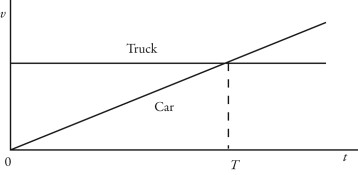
\includegraphics[width=0.5\textwidth]{figures/2_08.jpg}
%\begin{choices}
%   \choice The truck will have traveled further than the car.
%   \choice The car will have traveled further than the truck.
%   \choice The truck and the car will have traveled the same distance.
%   \choice The car will be traveling faster than the truck.
%\end{choices}

\question
\iftoggle{hideans}{\underline{~~~~~~~~~~~}}{\underline{~~~~~A~~~~~}}
The figure shows the velocity of a particle as it travels along the x-axis. What is the direction of the acceleration at t = 0.5 s?\\
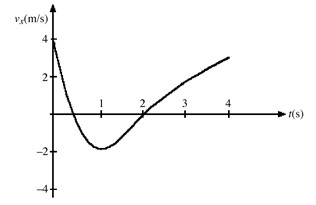
\includegraphics[width=0.45\textwidth]{figures/2_15.jpg}
\begin{choices}
   \choice in the -x direction
   \choice in the +x direction
   \choice The acceleration is zero.
\end{choices}

\question
\iftoggle{hideans}{\underline{~~~~~~~~~~~}}{\underline{~~~~~C~~~~~}}
Using the same figure as above, at what value (or values) of t is the instantaneous acceleration equal to zero?
\begin{choices}
   \choice t = 0
   \choice t = 0.5 s and t = 2 s
   \choice t = 1 s
\end{choices}

\question
\iftoggle{hideans}{\underline{~~~~~~~~~~~}}{\underline{~~~~~D~~~~~}}
A ball is thrown directly upward and experiences no air resistance. Which one of the following statements about its motion is correct?
\begin{choices}
   \choice The acceleration of the ball is downward while it is traveling up and upward while it is traveling down.
   \choice The acceleration of the ball is upward while it is traveling up and downward while it is traveling down.
   \choice The acceleration of the ball is downward while it is traveling up and downward while it is traveling down but is zero at the highest point when the ball stops.
   \choice The acceleration is downward during the entire time the ball is in the air.
\end{choices}

%\question
%\iftoggle{hideans}{\underline{~~~~~~~~~~~}}{\underline{~~~~A,C~~~~}}
%Under what condition is $\left|\vec{A} - \vec{B}\right| = A+B$? {\bf Choose up to 2 answers}
%\begin{choices}
%   \choice The magnitude of vector $\vec{B}$  is zero.
%   \choice Vectors $\vec{A}$  and $\vec{B}$  are in the same direction.
%   \choice Vectors $\vec{A}$  and $\vec{B}$  are in opposite directions.
%   \choice Vectors $\vec{A}$  and $\vec{B}$  are in perpendicular directions.
%   \choice The statement is never true.
%\end{choices}

\question
\iftoggle{hideans}{\underline{~~~~~~~~~~~}}{\underline{~~~~~D~~~~~}}
While an object is in projectile motion (with upward being positive) with no air resistance
\begin{choices}
   \choice the horizontal component of its velocity remains constant and the horizontal component of its acceleration is equal to -g.
   \choice the vertical component of both its velocity and its acceleration remain constant.
   \choice the vertical component of its velocity remains constant and the vertical component of its acceleration is equal to -g.
   \choice the horizontal component of its velocity remains constant and the vertical component of its acceleration is equal to -g.
   \choice the horizontal component of its velocity remains constant and the vertical component of its acceleration is equal to zero.
\end{choices}

%\question
%\iftoggle{hideans}{\underline{~~~~~~~~~~~}}{\underline{~~~~~C~~~~~}}
%For general projectile motion, when the projectile is at the highest point of its trajectory
%\begin{choices}
%   \choice the horizontal component of its velocity is zero.
%   \choice the horizontal and vertical components of its velocity are zero.
%   \choice its velocity is perpendicular to the acceleration.
%   \choice its acceleration is zero.
%   \choice its velocity and acceleration are both zero.
%\end{choices}

\question
\iftoggle{hideans}{\underline{~~~~~~~~~~~}}{\underline{~~~~~A~~~~~}}
A monkey is sitting at the top of a tree 20 m above ground level. A person standing on the ground wants to feed the monkey. He uses a bow and arrow to launch the food to the monkey. If the person knows that the monkey is going to drop from the tree at the same instant that the person launches the food, how should the person aim the arrow containing the food? Air resistance is small enough to be ignored.
\begin{choices}
   \choice He should aim it at the monkey.
   \choice He should aim it below the monkey.
   \choice He should aim it above the monkey.
\end{choices}

\question
\iftoggle{hideans}{\underline{~~~~~~~~~~~}}{\underline{~~~~~C~~~~~}}
A pilot drops a package from a plane flying horizontally at a constant speed. Neglecting air resistance, when the package hits the ground the horizontal location of the plane will
\begin{choices}
   \choice be behind the package.
   \choice depend of the speed of the plane when the package was released.
   \choice be over the package.
   \choice be in front of the package.
\end{choices}

\question
\iftoggle{hideans}{\underline{~~~~~~~~~~~}}{\underline{~~~~~A~~~~~}}
For an object in uniform circular motion, its velocity and acceleration vectors are always perpendicular to each other at every point in the path.
\begin{choices}
   \choice True
   \choice False
\end{choices}


%\question
%\iftoggle{hideans}{\underline{~~~~~~~~~~~}}{\underline{~~~~~B~~~~~}}
%A racecar is driving around a flat circular track at a constant speed $v_0$, at a radius of $r_0$. If he doesn't decrease his (centripital) acceleration he will roll his car. Which one of these methods would decrease his acceleration the most.
%\begin{choices}
%   \choice Increase his speed to $2v_0$.
%   \choice Decrease his speed to $\frac{1}{2}v_0$.
%   \choice Increase the radius of his path to $2r_0$.
%   \choice Decrease the radius of his path to $\frac{1}{2}r_0$.
%\end{choices}

\question 
\iftoggle{hideans}{\underline{~~~~~~~~~~~}}{\underline{~~~~~A~~~~~}}
If you set the cruise control of your car to a certain speed and take a turn, the speed of the car will remain the same. Is the car accelerating?
\begin{choices}
   \choice Yes
   \choice No
\end{choices}

% Worked problems
\newpage
\addpoints
\question[40] A hockey puck slides off the edge of a table with an initial velocity of 20.0 m/s and experiences no air resistance. The height of the tabletop above the ground is 2.00 m. What is the speed (not the velocity) of the puck just before it touches the ground? {\bf Make sure to show ALL work!}
\iftoggle{hideans}{~}{
\\~\\The first thing you want to do is recognize that the $x$ component of the velocity will remain constant so $v_{xi}=v_{xf}=20$ m/s since $a_x=0$ m/s$^2$. Then we need to solve for the $y$ component of the final velocity $v_{yf}$. This can be done by using one of the kinematic equations. The problem doesn't give you anything about time (though you can still use 2 equations, 1 to solve for time and then plug time into the other equation) so you probably want the equation
\begin{equation*}
   v_{yf}^2=v_{yi}^2+2a\Delta y
\end{equation*}
where $a=-g=-9.8$ m/s$^2$, $\Delta y = -2.00$ m as given in the problem and $v_{y_i} = 0$m/s. Plugging these in you get
\begin{align*}
   v_{yf}^2&=v_{yi}^2+2a\Delta y \\
   v_{yf}^2&=v_{yi}^2-2g\Delta y \\
   v_{yf}^2&=(0)^2-2*(9.8)*(-2.00) \\
   v_{yf}^2&=39.2 \\
   \rightarrow v_{yf} &= \sqrt{(39.2)} = 6.26 \text{ m/s}
\end{align*}

So now we know the components of the velocity
\begin{equation*}
   \vec{v}_{yf} = 20 \text{ m/s} \hat{i} + 6.26 \text{ m/s} \hat{j},
\end{equation*}
but we want the speed, which is the magnitude of the velocity. So we get
\begin{equation*}
   v_{yf} = \left|\vec{v}_{yf}\right| = \sqrt{20^2+6.26^2} = 20.96 \text{ m/s}
\end{equation*}
}

\end{questions}
\end{document}
